El modelo empleado es una arquitectura recurrente de inferencia de máscaras, basada en una LSTM que recibe la magnitud de la STFT de la mezcla y predice una máscara por fuente. Estas máscaras se aplican sobre la magnitud de la mezcla para obtener las magnitudes estimadas de cada \textit{stem}.
\begin{figure}[H]
    \begin{center}
    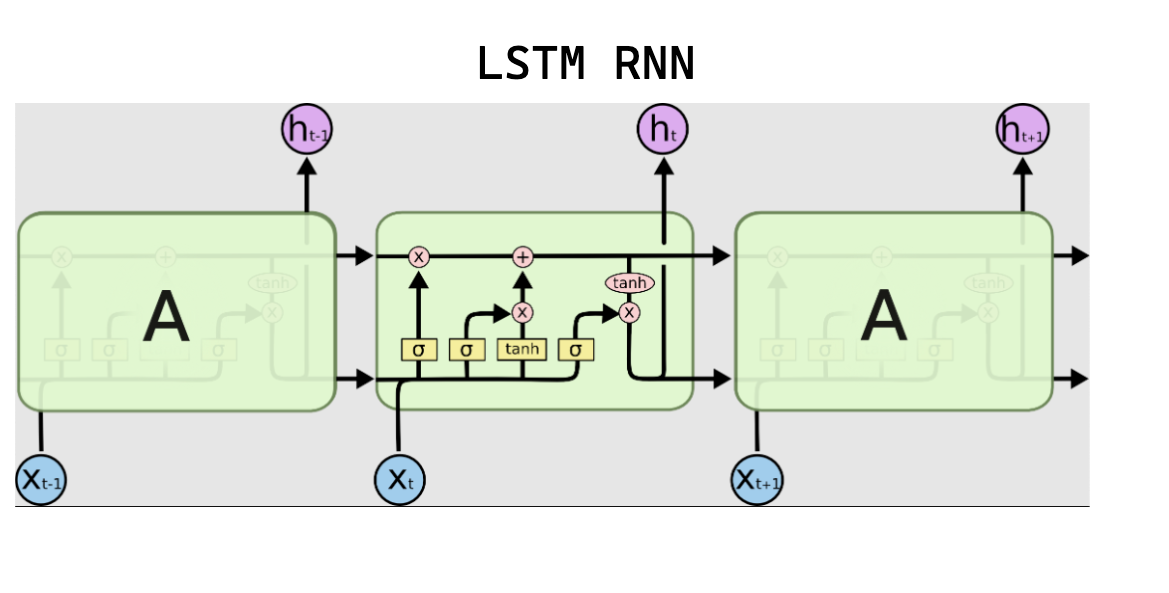
\includegraphics[width=0.7\textwidth]{commons/Fig9.png}
    \caption{Ejemplo de una arquictura RNN-LSTM}
    \label{fig:LSTM}
    \cite{rafii18}
    \end{center}
\end{figure}

En la figura se muestra una red neuronal recurrente LSTM desplegada en el tiempo.
Una LSTM procesa una secuencia paso a paso, palabras por ejemplo, sonidos o datos temporales.
Cada bloque verde representa la misma celda LSTM aplicada en diferentes momentos en el tiempo $x_{t}$ y $x_{t+1}$
$x_{t}$ es la entrada en el instante actual. 
$h_{t}$ es el estado oculto o salida de la celda en ese instante, lo que la red "\textit{entiende}" en ese momento


